\chapter{隐私保护}
\label{chap:trust-privacy}

为了检验邮件分类器对不同群体是否公平，开发者可能需要收集额外属性；为了提高识别能力，又可能希望使用私人邮件训练。模型发布后，即使原始邮件没有公开，输出和参数仍可能透露训练信息。数据后来被撤回时，删除存储中的记录也未必消除已经学入模型的影响。

在第~\ref{chap:trust-foundations}章的三层架构中，隐私保护主要属于系统属性或规范要求层：它规定谁的哪些信息可以被哪些主体以何种方式使用或获知。泄露审计、形式化分析与实现核查位于证据能力层；访问授权、数据流控制、重复发布的隐私会计和撤回处置，则需要在失效、处置与生命周期层落实。

要说明系统是否保护了隐私，需要先界定受保护的人、私人事实和泄露渠道，再确定可用什么证据检查这些边界。验证由此分为可见结果的泄露检验与处理过程的核查。保护措施按采集、训练和发布使用三个阶段安排；当数据使用许可被撤回时，还需分别处理数据副本与已进入模型的影响。公平审计中的群体越细，可能越容易发现集中伤害，也越容易暴露少量成员的信息；解决办法需要同时保留审计所需的证据，并约束信息可见范围，不能单独追求更细的统计或更少的数据。

\section{隐私保护的基本概念}
\label{sec:privacy-concepts}

\subsection{保护对象与保护范围}
\label{sec:privacy-subjects}

机器学习中的\term{隐私保护}（privacy protection）关注在完成任务时，如何限制个人信息被不适当访问、使用、推断或披露。保护对象不仅是提供训练数据的人，也包括正在提交请求的使用者，以及出现在邮件、图片或对话中的第三方。例如，用户提交一封邮件，邮件可能同时包含发送者、收件人和其他联系人的信息；确认提交者有权使用某个接口，并不能自动确定全部内容可以向谁公开。

需要保密的事实与保护单位应分别说明。这里的“秘密”是观察者试图获知的事实，例如“这封邮件参加过训练”、邮件里的私人编号，或推理请求中的地址。保护单位规定一次比较中允许改变多少数据，例如一条记录或一个用户的全部记录。换言之，秘密回答“要保护什么”，保护单位回答“机制限制谁的数据对结果的影响”，二者不是同一种分类。对单封邮件提供保护，不自动等于对同一用户一万封邮件提供同样强度的保护。

第~\ref{chap:trust-fairness}章用于比较误差的群体是评价单位，这里按记录或按用户界定的对象是保护单位；按群体报告效用损失，并不等于已经对整个群体建立同强度的隐私保证。还应说明同一个人的数据怎样被归集，以及记录中共同出现的其他人是否被所选单位覆盖，不能只按账户拥有者命名保护对象。

以下沿用一个受控例子：用户的一封邮件$z$含有私人项目编号，系统用一批邮件$D$训练分类器，并向外提供查询接口。需要分别考虑查询者能否判断$z$参加过训练、模型能否复现编号，以及训练服务器能否从共享更新恢复邮件。若该用户后来撤回全部邮件，删除范围还需要从单条$z$扩展为能定位到的全部相关记录及其衍生状态。

一项可核查的承诺应同时说明受保护对象、私人事实、使用目的、允许接收者和覆盖的系统接口。例如，允许模型为收件人整理邮件，不表示允许模型把其中的地址发送给无关工具。隐私保护应围绕这些边界展开，而不能只问训练数据是否曾经公开。

\subsection{机器学习中的泄露途径}
\label{sec:privacy-leakage-channels}

泄露可以发生在信息流的多个位置。采集、传输和存储阶段可能直接暴露原文；训练阶段可能通过梯度、检查点或调试日志暴露样本；模型发布后，参数和查询接口可能透露训练信息；推理时新加入的私人上下文，又可能流入检索结果、工具调用、回复和服务日志。调查时应逐处标明谁能够观察什么，不能只检查最终回答。

\term{成员推断}（membership inference）试图区分某条记录是否参与训练；属性推断利用可见信息推测未公开字段；数据重构尝试恢复输入内容；内容提取则可能通过多次查询诱导模型复现训练片段。这些名称描述泄露的私人事实或恢复方式，并不对应互不相干的处理阶段。例如，训练更新可以被用于重构，发布模型既可能被用于成员推断，也可能被用于内容提取。

模型并不需要逐字保存原文才可能泄露。对训练成员和非成员给出不同的分数模式，已经可能提供成员身份的线索；共同训练得到的参数也可能保留罕见片段。相反，模型正确判断一封邮件属于某类，可能只依靠一般语言规律，不能仅凭预测准确便认定它记住了该邮件。验证时要区分公开规律、观察者原有知识和使用私人数据后新增的信息。

训练数据本地保存只限制了原始数据的直接流转。如果参与者仍发布可逆的梯度或包含记忆的模型，信息可能从其他渠道流出。将原文换成向量、梯度或统计量改变了信息的表示，却没有自动建立保密性。访问权限、计算中间状态的可见性与最终结果所包含的信息，需要分别检查。

推理阶段的泄露也可能不涉及训练记忆。若用户刚提交的私人编号被模型转交给不应接收它的工具，即使模型从未用该编号训练，也已经越过了所声明的信息边界。一段内容出现在公开网页上，也不表示它适合在任何使用情境中再次披露。具体目的与接收范围仍需在第~\ref{sec:trust-context}节定义的情境中确定。

\subsection{保护承诺与强度}
\label{sec:privacy-guarantees}

对于直接访问，可以规定谁能够读取明文、执行哪些操作；对于共享计算，可以限制参与者看见哪些中间状态。但获准看见的统计量或模型仍可能透露私人事实，因此还需要约束发布结果对受保护对象的依赖。下面的差分隐私用于表达后一类承诺，并不替代全部访问与使用要求。

访问控制规定谁可以查询，却还没有说明获准查询者会知道多少。例如，某人已知除$z$以外的所有邮件，系统又发布包含某关键词的准确邮件数。若$z$含有该词，其加入就把计数从$c$变成$c+1$，查询者可以完全区分这两种情况。把结果称为“统计量”并没有消除单条记录的影响。

输出保护的一种思路是限制单个受保护对象对发布结果的影响。如果某个用户是否参与都只会小幅改变输出分布，攻击者就难以仅凭该变化确定其参与情况。\term{差分隐私}（differential privacy, DP）将这种要求写成对相邻数据集的比较。

\begin{definition}[差分隐私]
\label{def:privacy-dp}
给定与第一卷一致的相邻关系记号$D\sim D'$。若随机算法$M$对所有相邻数据集和所有可测输出事件$E$均满足
\begin{equation}
 \mathbb P(M(D)\in E)
 \leq e^\epsilon\mathbb P(M(D')\in E)+\delta,
 \label{eq:privacy-definition}
\end{equation}
则称其满足$(\epsilon,\delta)$差分隐私。这里$\epsilon\geq0$，$\delta\in[0,1)$，概率来自算法的随机性。
\end{definition}

回到计数例子，令$D$包含$z$，$D'$不包含$z$，并取输出事件$E=\{c+1\}$。若发布准确计数，则定义左侧为1、右侧为$\delta$，在$\delta<1$时不能成立。机制因此需要让两种数据下的可能输出有足够重叠，例如适当随机化发布值。定义只说明重叠需要达到什么程度，并未指定必须用哪一种加噪算法；机制负责实现定义，验证负责核对实现和证据。

相邻关系可以定义为增加或删除一条记录，也可以定义为替换一条记录；用户级保护则比较相差一个用户全部记录的数据集。选择相邻关系就是选择保护单位。较小的$\epsilon$和$\delta$限制更强，但$\delta$不是“每个用户以该概率被完全公开”的简单解释。

差分隐私限制参与数据带来的额外信息，并不阻止利用公开规律作出人口层面的推断。如果所有同类人群都具有某个属性，即使没有使用某个人的数据，也可能推测其属性。它也不保证任务输出正确。隐私定义、机制和组合分析需要一起理解\scite{dwork2014privacy}。

当$\delta=0$时，定义还可以通过假设检验理解。设$D$和$D'$只相差某条记录，检验在看到输出后决定“该记录参加了训练”，并把作出这一决定的输出集合记为$E$。在固定的这对数据集上，真阳性率$t=\mathbb P(M(D)\in E)$与假阳性率$f=\mathbb P(M(D')\in E)$满足$t\leq e^\epsilon f$；近似差分隐私则给出$t\leq e^\epsilon f+\delta$。这说明保证约束的是整条可行检验边界，而不是某个已知攻击的平均正确率。反向比较也受相邻关系的对称性约束。

由记录级保证推导群体变化时，参数通常会退化。若两个数据集相差$k$条记录，可以在它们之间插入$k-1$个中间数据集，逐次应用定义。由此得到
\begin{equation}
 \mathbb P(M(D)\in E)
 \leq e^{k\epsilon}\mathbb P(M(D')\in E)
   +\delta\sum_{j=0}^{k-1}e^{j\epsilon}.
 \label{eq:privacy-group-bound}
\end{equation}
这个推导表明，记录级保护可以推出群体界，却通常不能保持原来的参数。若一名用户最多贡献一百封邮件，直接把记录级$\epsilon$称为用户级$\epsilon$，会隐藏至多一百次相邻变化。限制每人贡献数量或直接按用户裁剪，才会改变需要分析的敏感度。

\paragraph{观察者与信任边界}

经典的中心化差分隐私允许可信的数据管理者先读取原始数据，再发布私有结果。若用户不愿让管理者看到明文，可以在发送之前就随机化信息，这称为\term{本地差分隐私}（local differential privacy）：任意两个可能的用户输入，都应产生难以区分的消息分布。它把保护放到数据离开用户的一刻，但每个用户独立加入的噪声需要共同进入统计估计。本地与中心化的区别在于谁可以接触明文；两者都可以采用差分隐私来约束指定接口的输出影响，不是两种互相排斥的隐私目标。具体的发送机制在第~\ref{sec:privacy-collection}节展开。

\section{隐私保护的验证}
\label{sec:privacy-verification}

确认泄露与证明保护成立，需要不同证据。从结果上检验，是让观察者在规定权限下尝试获得私人事实；这里的结果包括回复、分数、参数和可见更新，不仅是最终文本。从过程上核查，是检查信息如何流动，以及访问控制、随机机制和发布步骤是否满足承诺。结果检验可以揭示实际泄露，过程核查可以发现尚未被攻击利用的缺口；形式化保证还需要覆盖所有允许输入的论证。下面按这两类证据组织方法，再说明验证结论可以支持到什么程度。

\subsection{基于可见结果的泄露检验}
\label{sec:privacy-leakage-audit}

经验审计可以使用属性推断、成员推断、重构和提取攻击寻找泄露。审计必须固定攻击知识、查询预算、先验和评价数据，并区分随机猜测、总体规律与记录特有信息。如果成员和非成员来自不同时间或来源，攻击可能只识别了分布差异，未必识别训练成员身份。

审计方法应由秘密和可见接口共同选择：若秘密是未公开属性，就比较模型输出带来的额外推断能力；若秘密是某条记录是否参加训练，就检验成员身份；若关心发布模型能否复现私有内容，就尝试内容提取；若训练时共享更新，则检查更新是否足以重构输入。以下审计都要报告所恢复的信息、所需权限、误报及查询成本，而不能只报告一个含义不明的攻击成功率。

\paragraph{原文与字段的直接暴露}

有些泄露不需要复杂攻击：系统可能把邮件地址写入公开日志，或把工具无需接收的私人编号直接放进请求。可在隔离测试中使用合成私人标记，记录输入、模型回复、工具参数和可访问日志，逐项核对标记到达了哪些接收者。测试应涵盖不同账户权限和处理分支，并预先说明哪些流转是允许的。发现标记越过边界，可以确认这条路径存在泄露；没有发现，则只覆盖已经检查的路径。这类检查验证信息是否被直接交付，下面的攻击审计进一步检查没有直接交付原文时能否推断或恢复秘密。

\paragraph{未公开属性的推断}

若秘密是某个未公开字段，审计要检查模型输出是否让观察者比只使用其原有信息更容易推断该字段。例如，攻击者已经知道邮件主题和发送时间，希望推断未公开的项目类别；应分别训练只使用这些已知信息的基线，以及额外读取模型分数或表示的攻击器，再在同一来源的独立样本上比较。目标属性、攻击者先验、可见接口和查询预算必须固定，否则较高准确率可能只来自总体中某一类别本来就占多数。

这种比较得到的是接口是否增加属性推断能力的证据。即使模型从未见过目标个人的记录，人口层面的相关规律也可能支持推断；反过来，攻击器没有超过基线，只说明当前知识和预算下没有发现额外信息。报告应同时给出基线、各属性取值的错误、罕见群体表现和概率质量，而不能把一个平均准确率直接解释为私人属性已经暴露或得到保护。差分隐私限制参与数据带来的额外影响，不会自动消除从公开规律得到的属性推断。

\paragraph{训练成员身份的判别}

模型常对训练样本给出更低损失，但不同样本本来就有不同难度，不能用同一个置信度阈值充分区分成员与非成员。Shokri等人的工作使用影子模型模拟目标训练过程：在成员身份已知的辅助数据上训练模型，再学习其成员与非成员输出模式之间的差别。该工作说明，只有查询权限也可能得到成员证据；它并不要求攻击者直接读取目标训练集\scite{shokri2017membership}。

在有授权的受控审计中，可以把流程落实为以下步骤：
\begin{enumerate}
 \item 从同一来源准备候选数据，保存哪些样本实际进入目标训练集；将用于训练攻击器的数据与最终评价攻击的数据分开。
 \item 在辅助数据上训练影子模型，记录已知成员和非成员的损失、预测概率等输出特征，以成员标记训练攻击器。
 \item 对目标模型查询相同类型的特征。用验证数据确定攻击阈值，再在独立审计集上分别统计成员命中率与非成员误报率。
 \item 在固定查询预算下比较攻击器与不使用目标输出的基准，并报告低假阳性区域、候选成员先验和敏感子群的结果。
\end{enumerate}
这套流程把模型输出变成可验证的身份判断，而不是把某条记录的高置信度直接解释为训练记忆。

图~\ref{fig:trust-membership-inference}将候选记录、可见查询输出与成员判定分开。目标成员真值只在受控审计中用于核验；攻击器可以在辅助数据上学习规律，却不会因此得到目标训练集的成员名单。

\begin{figure*}[!htb]
  \centering
  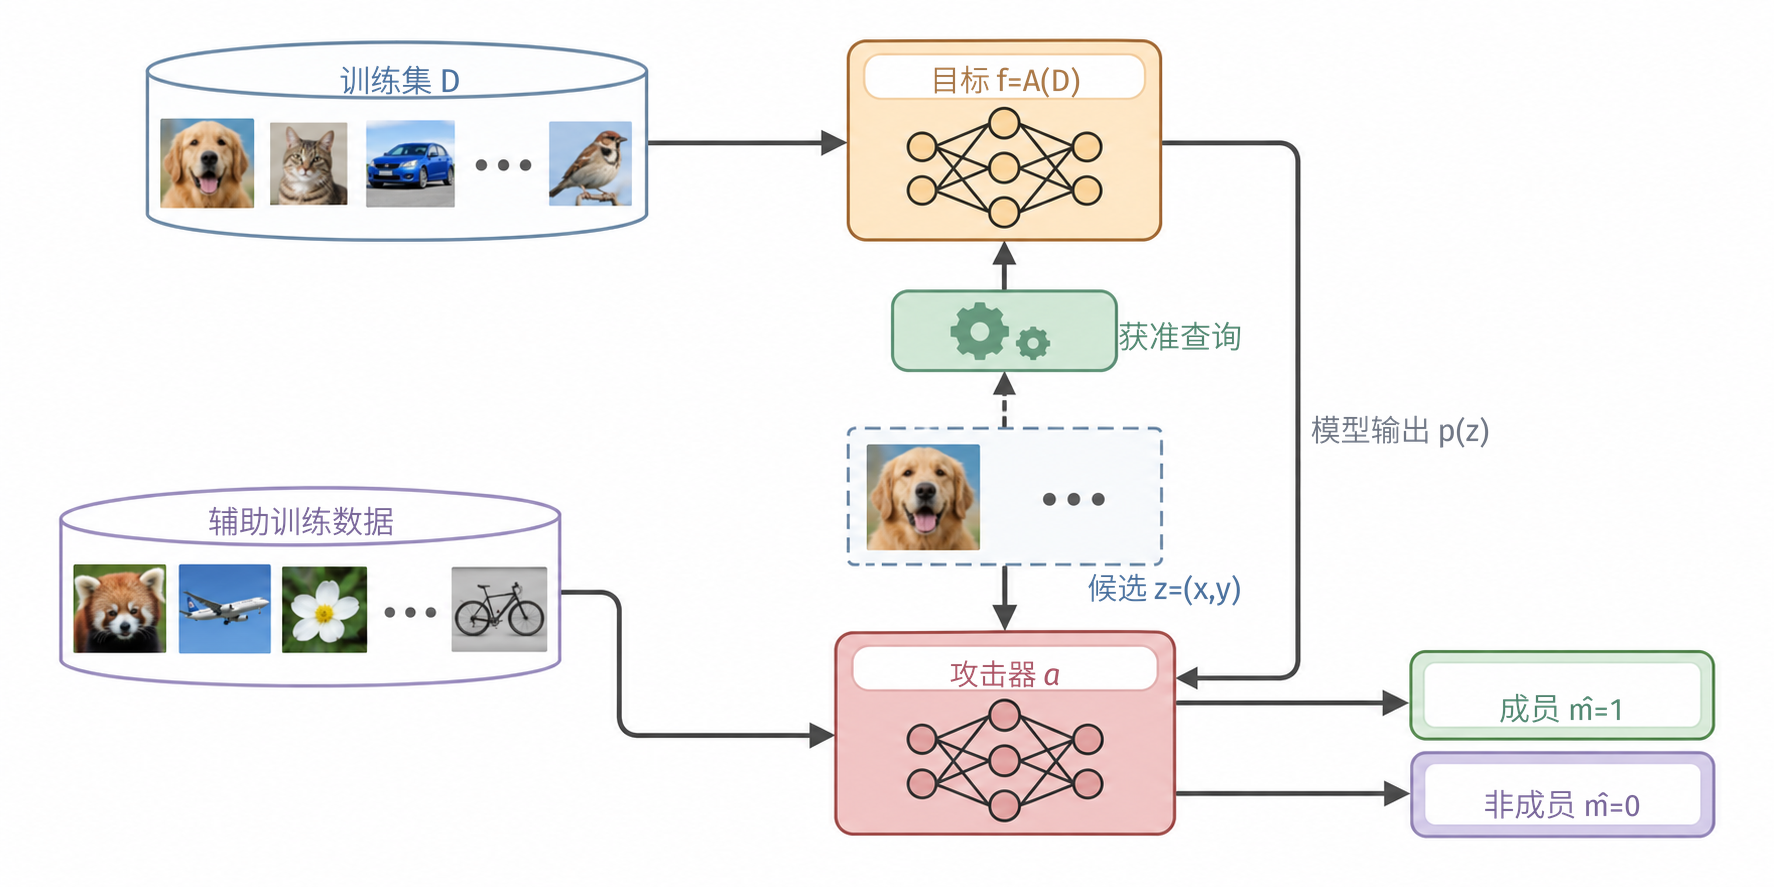
\includegraphics[width=164.600mm]{figures/02-foundations/03-trustworthiness/generated/membership-inference/figure.png}
  \caption{受控成员推断审计。本示意假定成员与非成员候选按同一分布抽取，目标模型仅以训练集$D$训练；候选记录$z=(\bm x,y)$通过获准接口取得输出。记录图标数量只表示分组，不代表成员先验。若真实标签$y$已知，可据此计算损失。攻击器由辅助成员数据训练，给出成员或非成员判定；完整审计还需在验证数据上确定阈值，并到独立审计集统计成员命中率与非成员误报率。目标成员真值只用于核验，不是攻击器输入。流程不保证攻击成功，权限、查询预算与成员先验须同时报告。}
  \label{fig:trust-membership-inference}
\end{figure*}

影子模型能够代表目标模型到什么程度，是这种审计的关键条件。若目标训练使用了不同的数据增强、早停或分布，辅助模型中学到的差别未必迁移。一个准确率较低的攻击也可能只针对少量异常敏感记录成功，因此总体平均值需要与个体、类别和低假阳性区域的结果一起报告。

Carlini等人的\term{似然比攻击}（Likelihood Ratio Attack, LiRA）将比较细化到单个待检验样本：用辅助训练估计“包含该样本”和“不包含该样本”时分数的分布，再比较目标分数更支持哪个假设。其研究强调在很低的假阳性率下报告真阳性率，并分析用变换后的置信度拟合分布的做法\scite{carlini2022lira}。

设样本$z$的观测分数为$s$，两个假设下的密度为$p_{\mathrm{in}}(s\mid z)$和$p_{\mathrm{out}}(s\mid z)$。理想化的检验统计量为
\begin{equation}
 \Lambda_z(s)=
 \frac{p_{\mathrm{in}}(s\mid z)}
      {p_{\mathrm{out}}(s\mid z)}.
 \label{eq:privacy-membership-likelihood}
\end{equation}
对两个完全指定的简单假设，似然比检验在给定假阳性约束下具有最优检验功效；该结论见
\BookTheoremRef{thm:statistics-neyman-pearson}{第一卷“随机变量”章的Neyman--Pearson定理}。
但实际审计只拿到有限辅助模型，密度估计有误差。该最优性不能直接变成经验攻击的无条件最优保证。逐样本比较的作用，是把“这条记录本来就容易预测”与“参与训练额外提高了它的可预测性”尽量分开。例如，同样观测到$0.95$的预测概率，对一条在“参加”和“未参加”两种情况下都容易预测的邮件，似然比可能接近1；对一条只有参加训练才经常获得该分数的罕见邮件，似然比才可能显著大于1。因此，影子模型攻击提供学习成员规律的一般流程，LiRA进一步规定了逐记录比较两种假设的方法，两者不应当作为完全无关的攻击类别理解。

\begin{example}[成员先验改变结果的含义]
\label{ex:privacy-membership-prior}
假设候选记录中只有$1\%$真正参加训练，一个审计检验的真阳性率为$0.8$、假阳性率为$0.1$。在一万条候选记录中，期望有80条真实成员被检出，同时有990条非成员被误报。检验报出的成员中只有约$7.5\%$是真的。这个教学例子说明，在成员与非成员各占一半的测试集上表现尚可，不代表在实际低先验场景中具有同样可信的阳性结果。
\end{example}

\paragraph{发布模型中的内容提取}

成员身份是一个二元事实，恢复内容则涉及更丰富的信息。Carlini等人研究了从语言模型输出中提取训练序列，区分了模型对文本赋予高概率与实际能够通过查询提取文本。其对GPT-2的实验表明，模型发布后可能复现训练片段，且不能只用平均泛化误差判断这种风险\scite{carlini2021extraction}。

提取审计必须把“生成了一个常见句子”与“恢复了训练中特有内容”分开。可以在受控训练中加入来源明确的合成标记，观察是否被重新生成；真实数据审计则需要来源核对、去重和对照语料。前者便于比较不同机制，却未必代表自然数据中的记忆；后者更贴近实际，但来源不完整时容易把公开重合、猜测与真正的训练信息混为一谈。测试报告应保留这些不同的证据强度。

对受控邮件例子，可以在训练前生成不含真实个人信息的唯一项目编号，把它只放入指定邮件，并保存不含该编号的对照语料。训练后预先固定一组提示、解码方式和每次完整试验的查询预算$k$，保存所有输出，统计一次试验内准确复现编号的次数。若采用随机解码，可在相同条件下用独立随机种子重复完整试验，再用至少复现一次的试验数除以总试验数，估计该预算下的提取成功率；确定性查询过程只报告其实际结果，不把重复相同输出当成新增证据。同时以未训练该邮件的模型或相应对照训练作为比较。若允许自适应修改提示，修改所用的查询也计入预算。这样得到的是指定查询策略下的可提取性，而非模型内部是否保存了该信息的完整判定。后续遗忘审计可以复用相同提示和预算，直接比较删除前后及重训练参照。

\paragraph{共享更新中的输入重构}

信息还可能在训练途中流出。Zhu等人的梯度深度泄露（Deep Leakage from Gradients, DLG）研究了已知模型和共享梯度条件下的数据重构：寻找能够产生相似梯度的候选输入与标签。其意义在于指出梯度仍是与私人样本相关的观测，而不是天然匿名的摘要；论文中的重构效果依赖模型、批次和所共享梯度等实验条件\scite{zhu2019dlg}。

以平方损失的线性模型作一个简化说明。单条记录的损失为$\ell=\tfrac12(\bm w^\top\bm x-y)^2$，则梯度为$(\bm w^\top\bm x-y)\bm x$。当残差非零时，即使未知其数值，梯度已经给出关于$\bm x$方向的约束；若额外共享偏置梯度，信息还会增加。这不是任意模型都能精确重构的证明，却足以解释“没有传原文”为什么不能推出“没有传原文的信息”。保护必须作用于实际可见的更新，而不能只检查网络请求中是否包含原始字段。

实际重构审计需要在受控数据上保留真实输入作为参照，并固定攻击者已知的模型、更新轮次、批次大小和辅助信息。评价应比较重构内容与真实输入，也与仅凭公开先验作出的猜测比较：图像外观相近、文本主题相近和精确恢复私人字段，是不同强度的结果。若攻击只恢复了常见结构，不能据此声称重构了特定记录；若少量私人字段已经准确恢复，也不能因整体重构误差较大而忽略泄露。

\subsection{基于数据流与实现的过程核查}
\label{sec:privacy-implementation-verification}

核查过程时，需要把承诺落实为数据流和执行条件。对于直接访问，检查实际采集字段、身份与权限校验、存储副本、日志、检索接口和工具接收者；对于统计保护，检查发布程序是否满足形式化机制的前提。前者能够发现原文绕过保护接口流出的路径，后者检查已获准发布的信息是否受到所声明的约束。

可以给同一封邮件建立处理清单：输入进入哪些存储位置，哪些人员或服务能读取它，经过什么变换，又产生哪些中间状态和外部输出。结合配置、实现和受控执行记录，检查拒绝访问是否实际生效、日志是否保留原文，以及备份和调试接口是否受到相同限制。仅审查一张流程图不足以确认运行中的程序遵守了这些约定。

验证差分隐私需要逐项核查保护单位、敏感度、噪声分布、抽样方式和组合过程。敏感度指改变一个保护单位能够使待发布统计量发生的最大变化，它决定需要多大的噪声。一个实现即使调用了“加噪声”函数，也不说明噪声已经按正确单位校准。例如，先按记录裁剪，却用用户级含义解释参数，会遗漏一个用户多条记录共同造成的影响。

参数选择、早停、超参数搜索和发布中间结果同样可能使用敏感数据。若这些环节没有被包含在分析中，最终模型的保证就可能不成立。实现检查还要覆盖随机数、日志和其他发布渠道；对一部分输出的证明不能自动覆盖系统另外写出的原始数据。

可把一次实现核验落实到同一个计数服务。若承诺是对增加或删除一封邮件提供纯$\epsilon$差分隐私，程序应先把每封邮件对关键词计数的贡献限定为0或1，再按敏感度1校准发布噪声，并记录同一数据还产生了哪些发布。这里不是仅核对配置文件里的$\epsilon$，而是沿着“原始输入如何变成计数、计数如何变成输出”核对每一步。

例如，一封邮件内重复出现关键词一百次，如果程序按词频累计，单条贡献就可能为100，原来的敏感度1论证不再适用。若仍按原尺度加噪，即使输出肉眼看来很随机，也没有实现所声明的保护。单元测试可以检查贡献截断、实际噪声尺度和重复发布记录，数学分析则需要覆盖所有允许输入；对几个样例测试通过不能替代敏感度的上界证明。第~\ref{sec:privacy-statistical-release}节将给出对应发布机制及推导。

对于安全聚合或加密计算，验证对象则是规定参与者能够观察什么、允许哪些串通以及协议依赖什么条件。计算过程被隐藏，并不约束最终公开统计量泄露多少信息。两类承诺应分别记录，再检查组合后的数据流。

\subsection{验证结论与适用边界}
\label{sec:privacy-verification-evidence}

同一个审计结果只能支持与实验对象相匹配的结论。在已经控制来源差异等混杂因素的条件下，成员推断的有效区分提供参与信息可被利用的证据；内容提取与重构则需要核实恢复内容的来源和特异性；它们不能不经转换就被当成同一强度的泄露证据。

攻击成功可以否定过强的保护主张；攻击失败只说明在所测攻击和资源下没有找到相应泄露。后者不能替代对所有输出事件的隐私定义。反过来，理论参数很大但某个攻击成功率很低，也不应把它解读为参数可以忽略。

经验攻击还可以反过来约束某个隐私主张的可信程度。在固定相邻数据对和检验事件的实验中，若真实真阳性率与假阳性率为$t,f$，且$t>\delta$、$f>0$，则差分隐私定义要求$\epsilon\geq\log((t-\delta)/f)$。但实验只能估计$t,f$，应使用真阳性率的置信下界与假阳性率的置信上界，不能把“没有观测到假阳性”直接当成$f=0$。普通成员与非成员分类实验若没有控制为相邻数据比较，也不能不经论证地套用这个反推。审计证据的含义取决于实验是否真正复现了定义中的比较对象。

评价还需要报告效用和成本。隐私机制输出完全无关噪声可以具有很强保护，却无法完成任务。不同群体的样本量和信号强度不同，噪声造成的效用损失也可能不同，因此应结合第~\ref{chap:trust-fairness}章进行分组检查。

公平审计需要使用敏感属性时，应把“审计所需访问”和“模型日常使用”分开。原始属性可以只在受限审计环境中由指定角色读取，用于计算预先声明的群体指标；训练服务和线上决策不因此自动获得同样权限。对外报告应限制到完成审计所需的统计量，并检查小分组、交叉查询和重复发布是否会暴露成员信息。最小组规模、访问控制和查询限流只能降低部分直接暴露，属于操作性缓解；若要承诺个体影响上界，还须限制每个用户的贡献、维护跨接口查询历史，并对联合发布采用与邻接关系匹配且可组合的隐私机制。验收也要分开进行：公平性证据检查重要群体是否仍有足够样本和有效分母，隐私证据检查谁读取了属性、发布了什么以及多次观察后的泄露边界。简单删除敏感属性会使公平差异无法测量，毫无限制地开放属性又会扩大暴露，两者都没有解决章首提出的取舍。

\section{隐私保护的实现}
\label{sec:privacy-use}

保护可以在私人信息进入系统前、转化为模型时，以及交付结果时实施。采集与存储措施决定哪些数据进入系统、谁能够直接读取；训练措施限制数据对参数和中间更新的影响；发布与推理措施约束接收者获得的信息，包括使用过程中新增的私人上下文。这些措施作用于不同位置，可以组合使用，不能用某一个阶段的保护代替全部阶段。下面每种机制都对应前节可以核查的数据流或输出承诺。

\subsection{数据采集与存储中的保护}
\label{sec:privacy-collection}

不收集无关信息可以减少需要保护的范围。必要信息也应明确使用目的、访问边界和保留时间。但这些措施并不替代输出保护：即使数据库访问受到限制，精确发布一人群体的平均值仍可能直接暴露个人值。

数据最小化需要落实到字段和任务。例如，邮件分类只需要正文的某些特征时，应先检验删除地址、私人编号等无关字段是否仍能完成任务，再决定是否采集或长期保存它们。若目的只需要设备上的预测，可以把处理留在设备上，并检查遥测与日志是否仍上传原文。不采集能够避免这条收集路径产生的风险，但删掉姓名或换成账户代号并不保证匿名：正文、时间和关联记录仍可能帮助识别个人。

对确有必要保存的信息，可以限制可访问角色、隔离用途、设置保留期限，并对传输和存储加密。加密主要限制没有相应密钥者读取内容；能够解密的处理方和最终接收者仍可能看到敏感信息。因此，需要同时控制解密后的使用和对外输出，不能把“数据库已加密”解释为模型不会泄露训练内容。

若确有收集需求，但接收者不应看到准确的个人值，可以在信息离开用户之前实施本地保护。这样改变的是接收者得到的输入；若接收者已经持有明文，之后才随机化发布，就属于不同的信任安排。

二元\term{随机响应}（randomized response）通过随机翻转私人位，在发送前限制其可辨识程度，也能说明保护如何影响统计精度。设私人位为$x\in\{0,1\}$，以概率$p=e^\epsilon/(1+e^\epsilon)$发送$x$，否则发送$1-x$。任一消息在两种输入下的概率比至多为$p/(1-p)=e^\epsilon$，所以满足本地纯差分隐私。若总体中$x=1$的比例为$\mu$，收到的位记为$Y$，则$\mathbb E[Y]=(1-p)+(2p-1)\mu$。当$\epsilon>0$时，可用$(\bar Y-(1-p))/(2p-1)$估计$\mu$；当$\epsilon$接近零，分母也接近零，估计误差被放大。强保护并不免费，这个简单例子把隐私与样本量、统计精度的联系直接暴露出来。

\subsection{训练过程中的保护}
\label{sec:privacy-training-influence}

模型训练要保留有用规律，又要限制单个对象如何改变发布模型。可以直接限制参数更新，也可以将私人知识限制在受保护的监督接口中。两种方式控制的信息通道不同，但最终都需要分析发布模型对相邻数据变化的可区分性。分析中的敏感度，是相邻数据变化能够造成的最大输出差异；限制这个差异，才能按明确尺度加入噪声。协作训练还需单独处理参与者看到的中间更新。

\paragraph{限制每次更新中的贡献}

训练算法通过许多更新累积单个样本的影响。\term{差分隐私随机梯度下降}（differentially private stochastic gradient descent, DP-SGD）通过限制样本梯度并对聚合结果加噪，构造可以进行组合分析的更新\scite{abadi2016dp}。

设批次大小为$b$，样本梯度为$\bm g_i$，裁剪阈值为$c>0$，则
\begin{equation}
 \begin{aligned}
 \bar{\bm g}_i
 &=\bm g_i\min\{1,c/\|\bm g_i\|_2\},\\
 \tilde{\bm g}
 &=\frac{1}{b}\left(\sum_{i=1}^{b}\bar{\bm g}_i+\bm Z\right).
 \end{aligned}
 \label{eq:privacy-dpsgd}
\end{equation}
零梯度约定仍为零，$\bm Z$为按所用隐私分析校准的高斯噪声。对于固定批次中替换一条记录，裁剪梯度和的敏感度至多为$2c$；增加或删除、抽样和用户级分组采用不同约定时，必须重新匹配敏感度与会计方法。随后用$\tilde{\bm g}$更新参数，并累计所有更新的隐私代价。

因此，一轮DP-SGD需要保留“逐样本”这个计算单位：先分别计算梯度，再分别裁剪，随后求和加噪，最后更新参数。若先把整批梯度相加再裁剪，得到的虽然也是有界向量，却不等于式~\eqref{eq:privacy-dpsgd}，不能直接沿用其逐样本抽样分析。训练结束只发布最终模型时，还须确认日志或中间检查点没有额外公开未受保护的梯度。

图~\ref{fig:dp-sgd-update}沿一次更新展示裁剪、聚合、加噪和参数更新的顺序；隐私账本还需累计多步更新的代价。

\begin{figure*}[htbp]
  \centering
  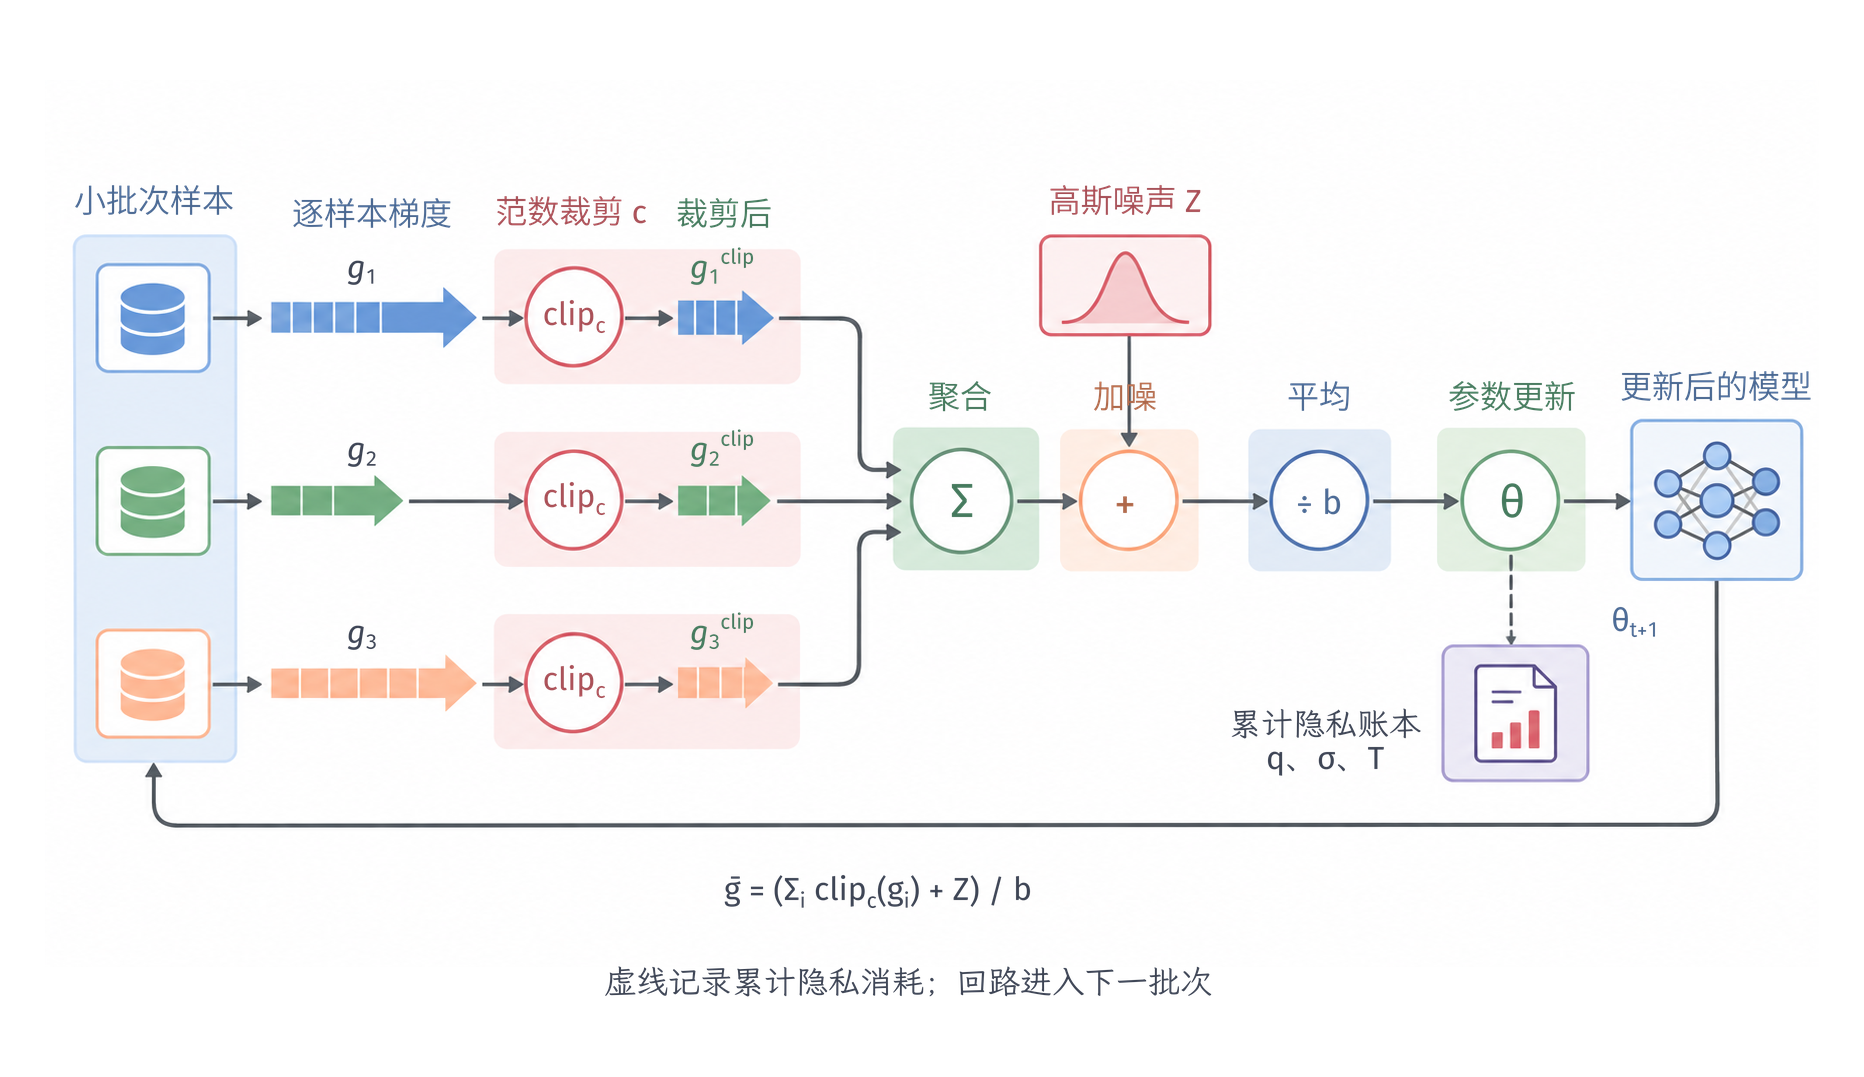
\includegraphics[width=164.600mm]{figures/02-foundations/03-trustworthiness/generated/dp-sgd-update/figure.png}
  \caption{独立计算批次内各样本梯度$\bm g_i$，先按阈值$c$裁剪：$\operatorname{clip}_c(\bm g_i)=\bm g_i\min\{1,c/\lVert\bm g_i\rVert_2\}$。裁剪后的梯度求和并加入高斯噪声$\bm Z$，再除以批次大小$b$并更新参数。隐私账本累计抽样率$q$、噪声尺度$\sigma$和更新步数$T$等条件下的消耗，需与保护单位、邻接和抽样约定匹配。向量长度与高斯曲线仅为机制示意。}
  \label{fig:dp-sgd-update}
\end{figure*}

裁剪防止单个样本无限影响更新，却可能引入偏差；噪声进一步降低可辨识程度，也会影响优化。训练轮数、抽样率和噪声强度共同决定预算。用户级保护通常需要限制一个用户的总贡献，不能只逐条裁剪后无条件相加。

更具体地说，可将高斯噪声写为$\bm Z\sim\mathcal N(\bm0,\sigma^2c^2\bm I)$，其中$\sigma$是相对于裁剪阈值的噪声乘子。若采用独立抽样，每个样本以概率$q$进入本次更新，批次大小是随机的，分母也应按实现和证明采用固定归一化常数或相应处理，不能直接套用固定$b$的公式。Abadi等人的DP-SGD通过裁剪、加噪与矩会计将深度网络训练中的多次访问纳入隐私分析；后续实现也常使用第~\ref{sec:privacy-repeated-use}节介绍的Rényi差分隐私会计，把多次更新的保护强度合并计算。

这里有两种容易混淆的效果。用$T$表示更新次数，固定$q,\sigma,T$及邻接约定时，按$c$同步缩放噪声，通常不改变由噪声与敏感度之比决定的隐私界，却会改变优化轨迹：$c$过小会使许多梯度被压缩，过大又会增加绝对噪声。增大批次也不必然改善隐私；它既改变每次平均更新的信噪比，也改变抽样率和完成既定轮数需要的更新次数，必须在相同训练预算口径下比较。

公开预训练模型上的私有微调提供了另一种效用来源。若预训练不使用本次受保护数据，只对后续私有访问进行会计即可；冻结一部分参数可能降低训练代价，但剩余更新仍需完整裁剪与分析。如果先用私有数据选择预训练模型、构造词表或筛除样本，这些数据依赖步骤不能因为发生在梯度下降之前就忽略。差分隐私承诺覆盖的是发布算法整体。

\paragraph{限制监督标签中的私人知识}

若直接对大模型每次更新加噪损失较大，可以让私有模型只提供少量受保护的监督。\term{教师集成的私有聚合}（Private Aggregation of Teacher Ensembles, PATE）把敏感数据拆成互不重叠的分区，每个教师只用一个分区训练；学生使用非敏感输入，并从教师的带噪投票中获得标签。私有接口是投票聚合，教师模型本身不发布\scite{papernot2017pate}。

设第$j$类票数为$v_j(\bm x)$，聚合可以发布$\arg\max_j\{v_j(\bm x)+Z_j\}$。在保持分区规则不变的条件下，更改一条记录最多改变一个教师的投票；一票从一类转到另一类，票数向量的$\ell_1$变化至多为2。这个敏感度限制来自教师之间的数据隔离，与每个教师是否采用凸优化无关。若同一用户出现在多个分区中，用户级影响则可能同时改变多个教师，原来的单位又不再适用。

教师意见一致时，一票改变通常不容易翻转答案；接近平票时，单票影响更值得警惕。可扩展PATE进一步采用高斯加噪聚合，并通过带噪的共识检查选择是否回答。它利用投票差距细化隐私分析，但是否通过阈值本身也与私人数据有关，必须计入代价\scite{papernot2018pate}。

拒绝低共识查询还会改变学生收到的训练分布。罕见邮件类型可能恰好更难形成共识，因而更少获得标签；这需要按群体检验获得监督标签的比例及学生模型的效用；标签获得比例并不是预测集合的覆盖率。PATE的操作顺序是先训练不发布的教师，再为事先说明来源的非敏感输入请求带噪标签，用这些标签训练学生；每次新增教师查询都产生需要计入的隐私访问。与DP-SGD相比，PATE把保护接口放在监督标签上，允许教师内部使用不同训练算法，但需要适合学生学习的非敏感输入，并承受查询数与共识不足的限制。DP-SGD直接在私有训练更新中限制影响，不依赖教师分片或这类输入。两者都需匹配保护单位，不能只比较最终噪声数值大小来判断谁保护更强。

学生训练只有在不再访问敏感教师或原始数据时才属于后处理。把学生继续放回私人数据上训练，会重新产生需要计入的访问。

图~\ref{fig:pate-private-teachers}展示私有教师与发布学生之间的信息边界：公开查询通过受保护的聚合标签参与学生训练，而私有样本不直接交给学生。

\begin{figure*}[htbp]
  \centering
  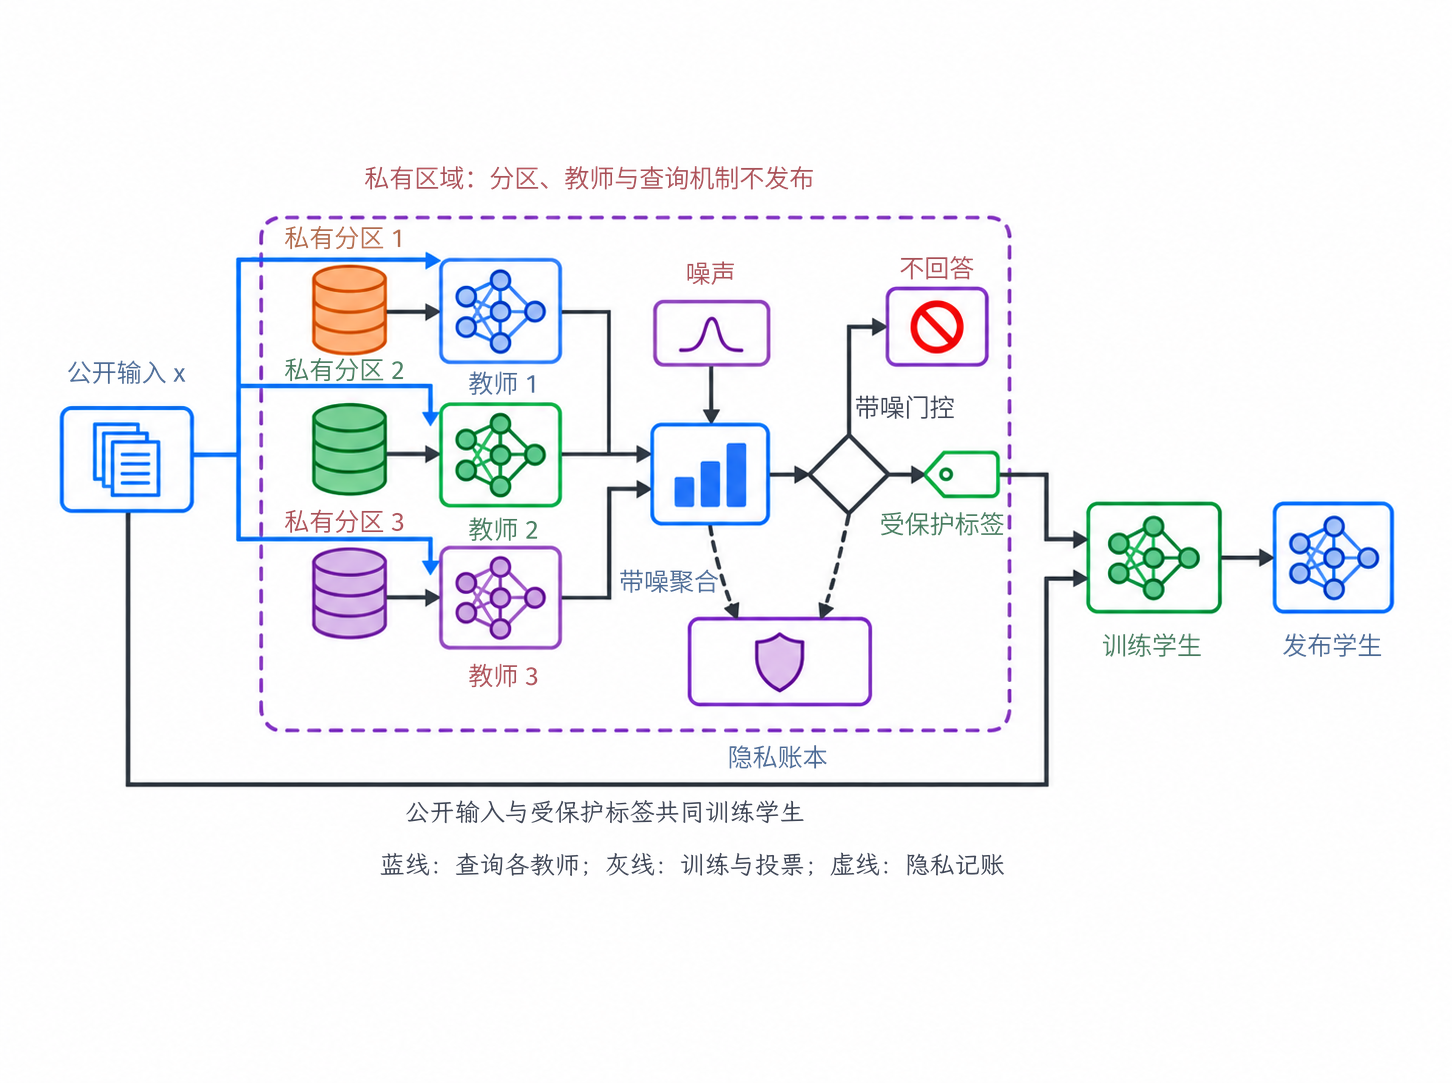
\includegraphics[width=164.600mm]{figures/02-foundations/03-trustworthiness/generated/pate-private-teachers/figure.png}
  \caption{互不重叠的私有分区分别训练不发布的教师。非敏感公开输入查询各教师，投票经加噪聚合和带噪门控后给出受保护标签，低共识时可以不回答。学生只使用公开输入和受保护标签训练并发布；私有样本与单个教师不进入学生。聚合与是否回答的决定均计入查询隐私代价。条形仅示意类别投票，不是测量结果。}
  \label{fig:pate-private-teachers}
\end{figure*}

\paragraph{协作方可见的中间更新}
\label{sec:privacy-collaborative-computation}

前面的机制约束发布结果对私人数据的依赖；参与训练的服务器或其他客户端还可能看到发布之前的更新。要保护这些中间观测，需要另行规定参与者的观察权限和串通范围。

安全聚合使服务方只能看到多个参与者的聚合结果，多方计算与同态加密可以在限制中间信息可见性的条件下完成指定计算，可信执行环境则依赖隔离执行和相应硬件假设。这些机制保护计算过程；如果最终模型仍记住私人内容，就还需要控制输出泄露。

Bonawitz等人的安全聚合协议面向许多客户端向服务器提交向量求和的场景。其基本思路是让客户端发送带掩码的更新，掩码在聚合中抵消，并处理部分客户端退出时的恢复需求。论文分别分析相应对手和串通条件，使服务器在规定条件下获得总和而非单个更新\scite{bonawitz2017secureaggregation}。

隐藏单个更新不意味着总和无害。若一个聚合只剩下一名未知贡献者，其余贡献都为观察者已知，总和就可能确定该贡献；多轮高度重叠的人群统计也可能产生差分信息。因此，安全聚合通常需要与参与人数、串通阈值和发布规则共同解释。它可以承载分布式加噪，但噪声由谁产生、多少诚实参与者留存、退出后总噪声是否仍充足，都属于新的证明条件。

图~\ref{fig:federated-learning-process}展示了本地记录、客户端更新与中心聚合之间的关系。原始记录留在设备上，上传的更新仍是与私人记录有关的观测，需要按本节的观察权限与串通条件检查。

联邦学习只是把训练计算分散到数据所在位置，并不自动回答这些条件。记录级DP-SGD保护本地某条记录，与对每个客户端总更新裁剪后建立用户级保证，也是两种不同方案。若中心服务器被信任，它可以在安全聚合后的总和上加噪；若不信任服务器，客户端需要在协议中共同提供足量噪声或采用其他信任安排。通信加密、聚合保密和统计输出保护应逐层连接，而不是互相替代。

\subsection{结果发布与推理使用中的保护}
\label{sec:privacy-statistical-release}

发布时需要检查接收者实际拿到什么。开放模型权重、提供受限查询接口和发布一张统计表，对观察者提供的权限不同。减少无关分数、原始记录和调试信息的返回，可以缩小直接暴露范围；限制接口与查询次数，也可以减少特定攻击获得的观察。但若没有相应分析，这些限制不能单独给出差分隐私保证。

\paragraph{发布统计量中的个体影响}

当可信管理者已经取得数据时，保护重点转为发布的统计量能透露多少个体信息。精确统计即使没有原文，也可能在小群体或多次差分查询中暴露个人值，因此需要对统计结果本身建立承诺。

设需要发布实值统计量$F(D)$，在既定相邻关系下的敏感度为
$\Delta F=\sup_{D\sim D'}|F(D)-F(D')|$。
敏感度描述一个受保护对象最多能改变多少输出。为隐藏这种差别，可以发布
\begin{equation}
 M(D)=F(D)+Z,\qquad
 Z\sim\operatorname{Laplace}(0,\Delta F/\epsilon),
 \label{eq:privacy-laplace}
\end{equation}
其中假设$\epsilon>0$且$\Delta F>0$。若敏感度为零，统计量本身不随相邻数据变化，无须为这一目的加噪。

式~\eqref{eq:privacy-laplace}满足纯$\epsilon$差分隐私。对任意输出位置$u$，两种数据下的密度比为
\[
 \exp\left(
 \frac{|u-F(D')|-|u-F(D)|}{\Delta F/\epsilon}
 \right)\leq e^\epsilon,
\]
不等式由三角不等式和敏感度定义得到。对输出事件积分即可得到式~\eqref{eq:privacy-definition}在$\delta=0$时的结论。这个推导也说明：噪声尺度由数据影响决定，不能任意选择后再解释为隐私参数。

图~\ref{fig:trust-dp-neighbors}用相差一条记录的计数说明随机化的作用。上部把准确计数与同分布噪声分别送入加法运算，下部显示由随机机制产生的输出分布。观察者拿到的是一次随机输出；保证约束两种可能数据下的全部输出事件，而不是要求这次输出相同。

\begin{figure*}[!htb]
  \centering
  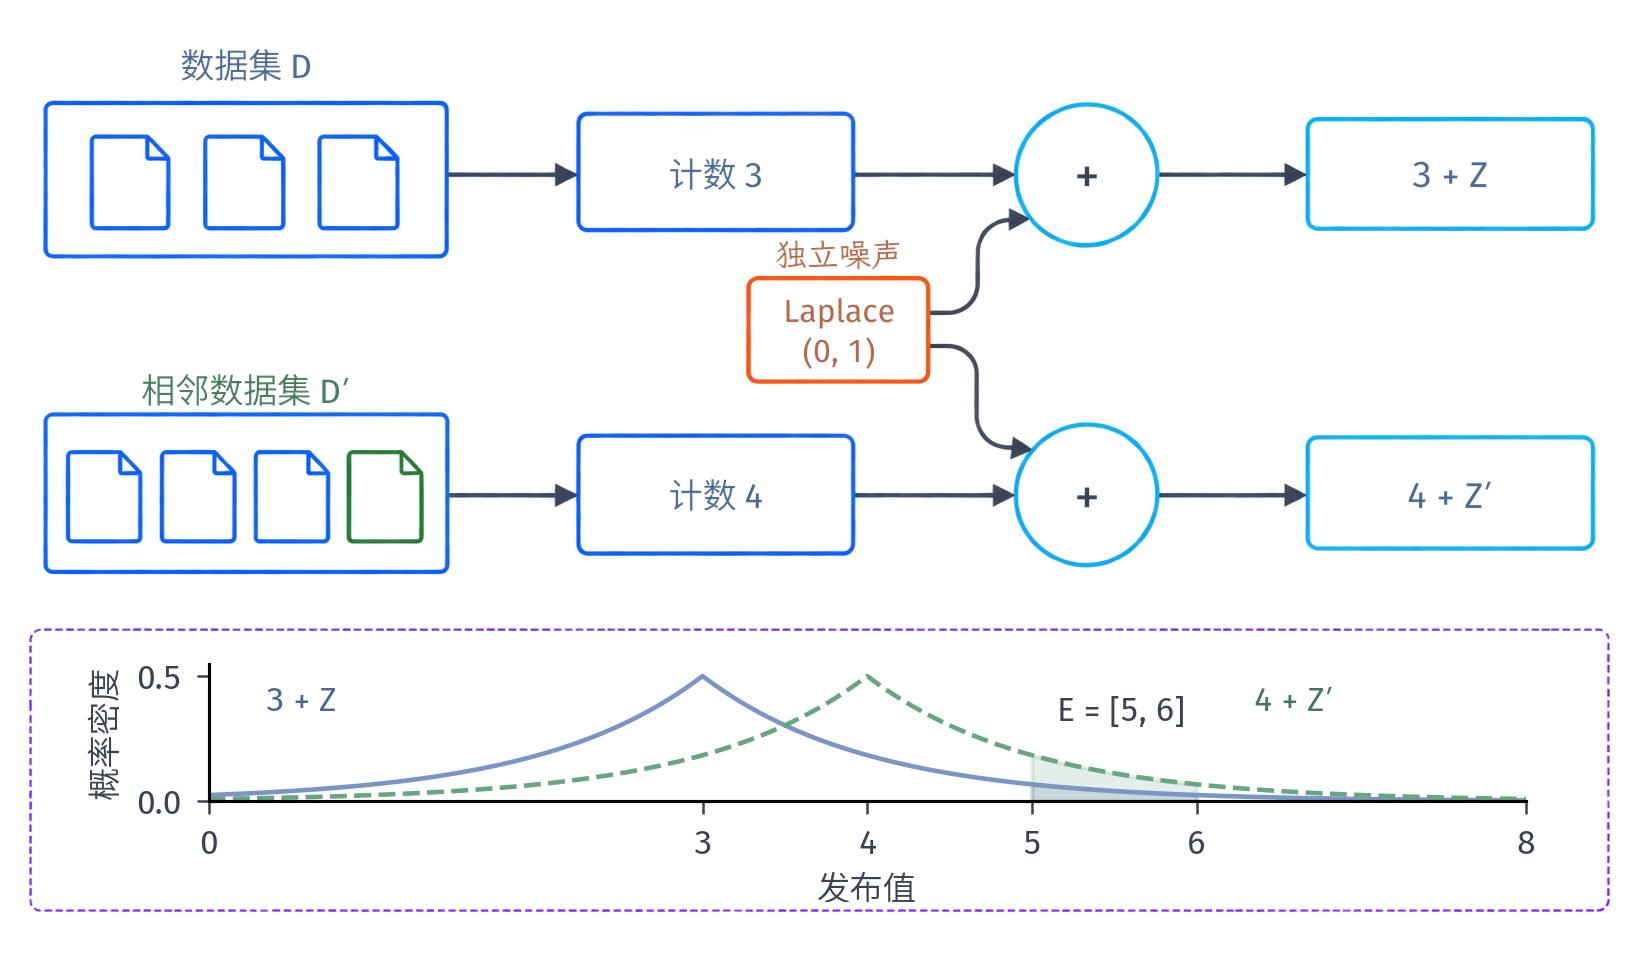
\includegraphics[width=164.600mm]{figures/02-foundations/03-trustworthiness/generated/trust-dp-neighbors/figure.png}
  \caption{相邻数据集与随机机制的输出分布。两组记录仅相差新增的一条，计数分别为3和4；每条路径各加一个独立的尺度1拉普拉斯噪声，对应$\Delta F=1$、$\epsilon=1$、$\delta=0$。加法节点显示噪声如何进入发布值；两侧是相邻数据的替代发布情形，不表示同时公开两次结果。下部实线与虚线是解析密度，阴影比较同一事件$E=[5,6]$的概率，横轴仅展示部分范围。观察者得到一次输出；隐私保证要求对所有相邻数据和所有输出事件成立，不能只看曲线重叠。}
  \label{fig:trust-dp-neighbors}
\end{figure*}

对前述关键词邮件数，记录级敏感度为1。若选择$\epsilon=0.5$，就向准确计数加尺度为2的Laplace噪声。真实计数相差1的两种数据会产生大量重叠输出，查询者不能再仅凭一个精确整数区分目标邮件是否存在。如果保护单位改为一个用户，而每人最多贡献10封相关邮件，计数敏感度变为10；保持相同$\epsilon$需要尺度为20的噪声，除非重新设计贡献限制。这些数值只是定义和机制的代入，显示保护单位、效用损失与实际实现如何相连。

\begin{example}[计数与平均值的不同要求]
\label{ex:privacy-sensitivity}
按增加或删除一条记录定义相邻时，人数计数的敏感度为1。若发布固定$n$条记录中数值的平均值，按替换一条记录定义相邻，且每条数值预先限制在$[0,1]$，敏感度为$1/n$。去掉取值界后，均值敏感度可能无界。两种例子使用不同相邻约定，必须分别写清。
\end{example}

\paragraph{推理上下文与结果接收者}
\label{sec:privacy-inference-context}

推理阶段也有独立的信息流。检索私人文档、调用工具和记录对话日志，可能将敏感内容带到新的边界。应只提供完成任务必要的上下文，限制工具返回字段，并对输出对象和接收者进行检查。对私人上下文提供形式化保护时，每次新访问都应纳入相应机制的分析。

这里的保护对象是当前请求中的私人信息，而非仅限于训练记录。一个已经具备训练数据差分隐私保证的模型，如果收到私人邮件后原样转交外部工具，仍然可能泄露该请求。应在上下文进入模型、工具接收字段和结果交付接收者这几处分别明确边界；训练阶段的保证不会自动覆盖新增输入。

实际控制可以从检索前的权限检查开始：仅让当前用户有权访问的文档进入上下文，按工具任务裁减字段，对回复和工具请求检查接收范围，并限制日志保存内容。输出过滤能够拦截已知标识或特定模式，但可能遗漏改写和间接推断，也可能误删合法内容，应该通过前节的结果检验与过程核查分别验证。过滤有效不等于私人上下文已经获得形式化保护。

\paragraph{多次发布的累计保护强度}
\label{sec:privacy-repeated-use}

若已经发布$M(D)$，再用不访问原始数据的随机过程处理它，不会增加差分隐私参数。这称为后处理性质：对处理后任一输出事件，可以把它追溯为原机制输出上的一个随机检验，并继续应用式~\eqref{eq:privacy-definition}。

如果重新访问数据运行多个机制，情况不同。基本组合界将每一步的$\epsilon$与$\delta$分别相加；更精细的会计可以利用机制结构获得更紧的界，但不能忽略重复试验和模型选择。对已发布私有模型作纯后处理查询，与每次查询都重新读取私人上下文，是两种不同的信息使用过程。

只要多次发布都依赖同一个受保护对象，就需要计算联合观察下的保护强度。下面给出训练和持续服务中可用的组合分析。它适用于前述各阶段，不是一个额外的数据处理阶段。

以$\epsilon=0.5$的关键词计数服务为例，对同一批邮件重新抽取噪声并发布三次，基本组合给出$1.5$的纯差分隐私上界；若只是把已经发布的一次带噪计数画成图、转换单位或重复显示，则属于后处理，不增加这项预算。若三次调用来自不同网页或不同功能，只要它们读取的是同一个受保护对象，也不能因此分开忽略。累计分析针对观察者能够联合看到的结果。

训练往往包含成千上万次更新，逐步转换为$(\epsilon,\delta)$再相加可能过于保守。
Rényi散度及逐历史统一条件下的自适应组合已经在
\BookDefinitionRef{def:information-renyi-divergence}{第一卷“信息论与统计几何”章的“Rényi散度”定义}
与
\BookSectionRef{sec:information-sequential-accumulation}{同章的“序列信息累积”一节}
建立。本章只增加隐私邻接和机制条件。\term{Rényi差分隐私}
（Rényi differential privacy, RDP）要求对所有相邻数据集，输出分布满足相应阶数的
Rényi散度上界。沿用第一卷记号，对概率分布$P,Q$和$\alpha>1$，
\begin{equation}
 D_\alpha(P\|Q)=\frac{1}{\alpha-1}
 \log\mathbb E_{o\sim Q}
 \left[\left(\frac{\mathrm dP}{\mathrm dQ}(o)\right)^\alpha\right].
 \label{eq:privacy-renyi}
\end{equation}
若对所有相邻数据集，该量均不超过$\rho(\alpha)$，就得到相应阶数的RDP保证。绝对连续性
与无穷值约定沿用第一卷。Mironov建立了这种隐私定义及其组合、后处理和转换性质
\scite{mironov2017rdp}。

若第$t$次机制在给定此前输出后仍满足统一的RDP界$\rho_t(\alpha)$，则组合界为$\sum_t\rho_t(\alpha)$。对事先指定的$\delta\in(0,1)$，一个有效的转换结果是
\begin{equation}
 \epsilon(\delta)=
 \inf_{\alpha>1}\left\{
 \sum_{t=1}^{T}\rho_t(\alpha)
 +\frac{\log(1/\delta)}{\alpha-1}
 \right\}.
 \label{eq:privacy-accounting}
\end{equation}
上式中的最小化是在已经证明有效的阶数界之间选择，不需要再访问私人数据。例如，不含抽样的高斯发布机制具有$\rho(\alpha)=\alpha\Delta_2^2/(2s^2)$，其中$\Delta_2$为向量统计量的二范数敏感度，$s$为各坐标噪声标准差。训练中的抽样会改变这条曲线，必须使用相应抽样机制的分析，不能把抽样率随意乘到最终$\epsilon$上。

\section{数据撤回与模型消除}
\label{sec:privacy-unlearning}

本节的模型消除主要指消除指定数据在模型中的训练影响，即\term{机器遗忘}（machine unlearning）；删除或停用整个模型是另一种操作。删除数据库中的记录、阻止某段文本出现和消除训练影响，具有不同的验收对象。

记训练算法为$A$，原数据为$D$，待撤回记录集合为$F$，模型更新程序为$U$。图~\ref{fig:trust-privacy-deletion}把删除后的数据与模型更新分开。清理数据不会自动改变先前训练的模型；消除训练影响需要将更新结果与从未使用撤回记录的重训练结果比较。未能提取私人片段，也不能仅据此认定训练影响已经消除。

\begin{figure*}[htbp]
  \centering
  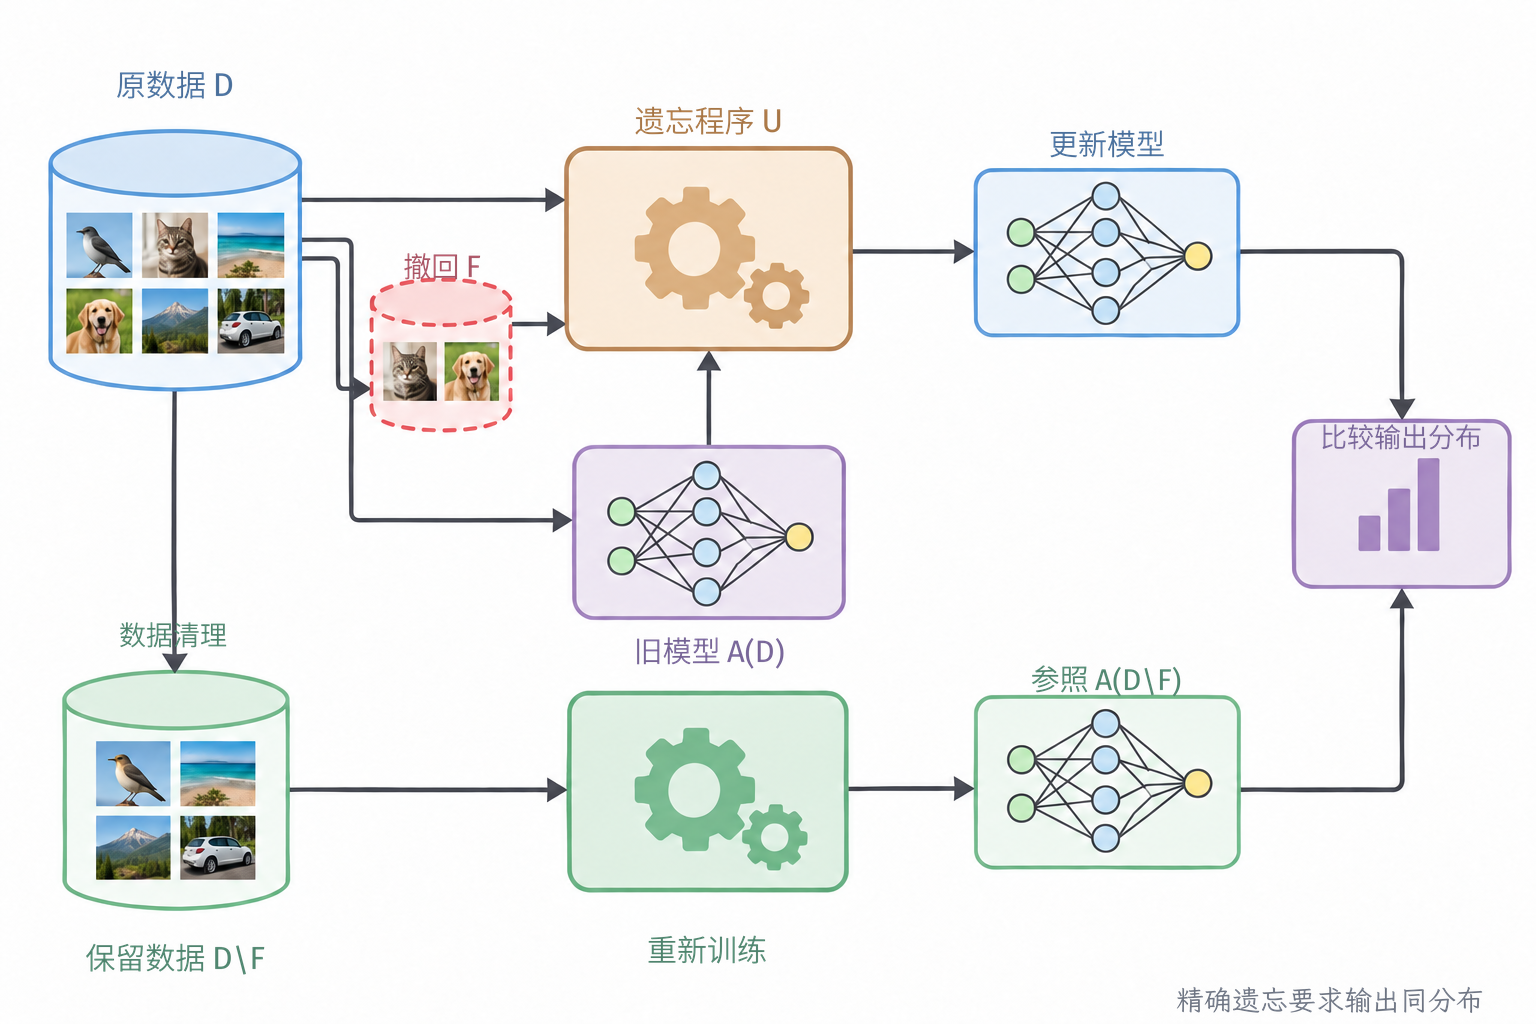
\includegraphics[width=164.600mm]{figures/02-foundations/03-trustworthiness/generated/unlearning-reference/figure.png}
  \caption{撤回记录与消除训练影响的两条路径。清理数据得到$D\setminus F$，旧模型$A(D)$不会因此自动改变；更新程序$U$另行读取旧模型、原数据和撤回集合。更新结果与从未使用$F$的重训练参照比较输出分布；精确遗忘要求同分布，近似遗忘须声明距离或可区分性标准。}
  \label{fig:trust-privacy-deletion}
\end{figure*}

在集合差按记录身份处理的约定下，先限定观察者只能取得替换后新发布的模型，不保留
旧模型、旧回答、训练日志或其他辅助状态。在这个观察视图内，精确遗忘要求更新程序$U$满足
\begin{equation}
 U(A(D),D,F)\ \overset{\mathrm d}{=}\ A(D\setminus F).
 \label{eq:privacy-exact-unlearning}
\end{equation}
这里$\overset{\mathrm d}{=}$表示新模型的输出分布相同，概率包含训练与遗忘算法的随机性。
右侧是从未使用撤回记录的重训练参照。若观察者还能联合看到旧模型、旧回答或辅助状态，
就必须比较相应的联合观察分布；新模型边缘分布相同不能撤销已经披露的信息。实际程序可以
使用额外保存状态，但这些状态一旦对观察者可见，也必须纳入比较。

近似遗忘允许两种分布在指定距离或可区分性标准下接近。必须说明比较对象是参数、预测行为还是某类攻击结果；只在少量问题上不再输出原文，不能推出参数分布已经接近重训练。

差分隐私与遗忘也不等价。前者在训练时限制一个对象对输出的影响，后者在撤回后与特定重训练结果比较；二者可以配合，但不能仅凭训练使用了差分隐私便宣称完成了任意撤回要求。

一次撤回不等于任选一种操作。每项请求都要先确定撤回范围，停止相关数据继续被正常使用，清理可控制的数据副本与衍生状态，并隔离暂时无法清除的部分。若撤回数据已经影响训练结果，还需从完整重训练、局部重算和参数修正中选择满足既定遗忘标准的路线；三者是备选方案，不是需要依次执行的步骤。撤回的正式处置完成前，输出限制只能作为过渡保护。最后还要统一验收数据资产、服务接口和模型影响，并报告完整流程的时间与资源代价。

\subsection{撤回范围与数据资产清理}
\label{sec:privacy-asset-deletion}

撤回从定位范围开始。应根据稳定的记录标识、用户与记录的关联，以及处理过程留下的依赖关系，找出原始文件、清洗副本、特征缓存、检索索引、向量记录、训练快照和相关日志。对用户级撤回，不能只删除账户表中的一行；对包含多个人信息的共同记录，还要说明本次实际删除的是整条记录还是其中的字段。

减少响应时间的关键是事先能够查出数据去向。可以维护记录到数据版本、索引条目、训练任务和模型版本的映射，按这份映射生成撤回任务。请求确认后，先阻止相关数据继续进入训练队列、检索结果和新的副本，再按存储与依赖清单安排各位置的清除或重建，并检查正在运行的任务是否仍持有旧快照。删除标记只表示数据不可再被正常使用，与物理副本已经清除是两种完成状态。

清除顺序还要与模型更新协调。后文的贡献扣除需要计算撤回记录的统计量，部分参数更新也需要在撤回样本上计算损失；这些计算若依赖原始内容，就应在受限的撤回处理环境中完成，再清除相应工作副本。也可以在已有状态足够时直接使用必要统计量，但这些状态本身仍须检查是否含有私人信息。先停止正常训练与检索中的使用，不等于必须先销毁遗忘算法尚需读取的全部输入；临时副本的访问范围、存续时间和最终删除，都属于同一次撤回的验收范围。

索引删除尤其需要检查派生缓存。例如，移除文档后，其向量、缓存片段和已生成的摘要仍可能被检索或复用。备份恢复也应重新应用撤回记录，避免已经删除的数据在恢复后重新进入服务。若某些归档不能立即逐条清除，应明确其隔离措施、清除安排和恢复限制，不能把在线不可见写成所有副本已经消失。

验收时应按存储和依赖清单核对已完成、待完成与无法控制的副本，测试撤回记录是否仍能被检索、导出或再次进入训练，并记录涉及的模型版本。日志应能证明处置过程，同时避免为了审计重新保存完整私人内容。数据资产清理完成，只解决系统仍保存或重新使用什么；已经写入参数的训练影响还需选择下面的消除方案。

\subsection{训练影响的消除方案}
\label{sec:privacy-unlearning-methods}

数据进入训练结果后，需要选择与遗忘标准、算法结构和可用状态相匹配的消除方案。完整重训练直接构造参照；局部重算利用可追踪的计算依赖减少工作量；参数修正则从现有模型出发逼近删除后的结果。三条路线的适用条件和证据强度不同，不能把计算量较小直接解释为遗忘更充分。

\paragraph{完整重训练}

最直接的方法是排除撤回集合$F$，在$D\setminus F$上重新执行训练算法$A$。这条路线直接构造式~\eqref{eq:privacy-exact-unlearning}右侧的参照，代价是重新处理保留数据与训练模型。这里的参照是同一训练流程在保留数据上产生的模型分布，不要求恰好复现某一组随机参数。

完整重训练还包括受撤回数据影响的前置步骤。若词表、特征标准化、样本筛选或模型选择曾使用$F$，就应重新计算这些依赖；若优化器状态或初始化检查点已经受$F$影响，直接从该状态继续训练也不等于从未使用$F$。只有确认独立于撤回数据的公开预训练模型或中间结果，才可以作为可复用起点。提前停止的轮数、随机抽样规则与其他训练约定也属于$A$的一部分。

重训练后需要切换服务版本、失效旧缓存，并清楚标识新模型覆盖了哪些撤回请求。多项请求可以合并重训以减少重复计算，但等待期间仍需要限制旧数据与旧服务的暴露，且必须报告实际等待时间。批量处理改变的是效率，不能把“已经进入下一批任务”写成模型影响已经消除。

\paragraph{局部重算}

要比完整重训更快，需要知道撤回数据影响了哪些计算。若模型只依赖可更新的统计量，可以扣除被撤回记录的贡献；若训练事先被隔离为若干部分，可以仅重算受影响的部分。节省来自明确的计算依赖，而不是从任意神经网络参数中直接找到一条数据对应的位置。

当训练结果由可更新统计量决定时，可以直接扣除撤回记录的贡献。Cao和Yang研究把学习过程组织为可更新的求和形式，在撤回时修改相关统计量，以减少重新处理全部数据的代价。这种思路要求算法与数据处理确实具有相应结构，并需要追踪衍生数据的依赖\scite{cao2015unlearning}。

设一个教学估计器只通过记录数$n$与数值和$S$得到均值$\hat\mu=S/n$。若撤回$m<n$条记录，其数值和为$S_F$，则更新为
\[
 \hat\mu_- =\frac{S-S_F}{n-m}.
\]
这与对保留记录重新计算均值在数学上相同，只需取得撤回集合的贡献；数值实现仍需考虑浮点误差。例如原数据为$1,2,3$，撤回3后，直接更新得到$(6-3)/(3-1)=1.5$。这说明在特定模型中可以通过更新状态精确移除贡献，但不意味着深度网络也能把某个样本的训练梯度简单减回去：后续更新依赖先前参数，通常会受到连带影响。

若计算依赖在训练前已经隔离，局部重算还可以只触及受撤回记录影响的部分。SISA训练把计算依赖组织为分片、隔离、切片与聚合（Sharded, Isolated, Sliced, and Aggregated）：各分片独立训练子模型，分片内部按切片逐步训练并保留检查点，最终聚合子模型预测。撤回一条记录时，从该记录首次进入训练之前的检查点恢复，只重新训练受影响的后续部分。它用事前隔离换取撤回时的局部重算\scite{bourtoule2021sisa}。

例如，把邮件按预先固定的规则分到四个分片，每片分成三个顺序切片。某条待删除邮件只位于第二分片的第二切片，则其他三个子模型无需变化，第二分片第一切片结束的状态可以保留，后两片在排除该邮件后重算。这一教学例子中的节省来自依赖关系，而不是算法能够从任意最终参数中抽出一条记录的影响。如果特征标准化、词表或模型选择在全部数据上共同完成，仍可能留下跨分片依赖，必须纳入撤回流程。

分片越多，每个子模型可用的数据越少，集成预测与整批训练也可能具有不同效用；检查点越密，存储和敏感状态管理代价越高。因而不能只比较一次删除的耗时。应同时比较初始训练、状态保存、常见删除批量、最坏删除分布和保留任务的效果，并固定重训练基线的算法。

这里的局部重算应与同一分片、切片和聚合规则下的重训练比较，并核对数据移除后抽样与随机状态的处理是否一致。与一个从头训练的整批单模型相比，SISA本来就是另一种训练算法，不能据此宣称二者输出分布相同。

\paragraph{参数修正与近似遗忘}

如果没有预先隔离所有依赖，可以尝试从已有参数出发逼近删除后的模型，但“修正得很小”与“删除得充分”没有必然关系。

一种参数修正路线为近似误差给出理论控制。Guo等人的认证数据删除针对有正则化的线性模型，利用牛顿更新近似删除后的解，再用训练时的目标扰动隐藏剩余误差。其保证依赖强凸性、平滑性等条件；仅有很小的梯度残差并不能独立证明删除成功\scite{guo2020certifiedremoval}。

这个机制可以用优化残差理解。设原参数为$\hat{\bm\theta}$，删除后的光滑强凸目标为$L_-(\bm\theta)$，在原参数处的梯度和海森矩阵分别为$\bm g_-$和$\bm H_-$。一步牛顿近似为
\begin{equation}
 \tilde{\bm\theta}
 =\hat{\bm\theta}-\bm H_-^{-1}\bm g_-.
 \label{eq:privacy-newton-removal}
\end{equation}
若删除后目标在局部接近二次函数，这一步能消除主要的一阶偏差；剩余误差可用$\|\nabla L_-(\tilde{\bm\theta})\|_2$描述。但确定性的微小误差仍可能携带记录信息，因为观察者可以检查非常精细的参数差别。认证方法还需要把残差界与随机扰动分布连接，证明删除输出与重新训练输出在指定可区分性标准下接近。

强凸性给出的是一个相关但较弱的结论：对无约束可微目标，若强凸参数为$\lambda>0$、真正最优解为$\bm\theta_-^*$，则
$\|\tilde{\bm\theta}-\bm\theta_-^*\|_2
\leq\|\nabla L_-(\tilde{\bm\theta})\|_2/\lambda$。
它说明优化误差可以由残差控制，却还不是输出分布的隐私界。连续撤回时，残差和认证预算需要累积；当条件超出允许范围，重新训练是恢复承诺的一种方式。把针对强凸线性模型的推导直接套到大规模非凸语言模型，会丢失决定认证是否成立的关键前提。

对不满足上述认证条件的深度模型，也可以采用经验更新：在撤回数据上提高预测损失，使模型降低对相应答案的概率；同时在保留数据上继续降低任务损失，或约束模型在这些数据上的预测变化。前一项促使模型遗忘，后一项限制附带损伤。若不使用保留约束，只反复提高撤回损失，模型可能通过破坏大量能力达到这一目标，因而不能把撤回集准确率越低理解为遗忘越充分。

负偏好优化（Negative Preference Optimization, NPO）研究了语言模型遗忘中的这一不稳定性。它以原模型作为参考，用目标序列在当前模型与参考模型下的相对概率调节遗忘更新；当某个目标已经被明显压低后，其更新权重随之减小。该目标可以与保留数据的训练损失结合，以限制效用损失。它提供了一种调整参数的经验路线，并不自动证明任意语言模型已接近完整重训练的参数分布\scite{zhang2024npo}。

第~\ref{sec:interpretability-local-training}节中的局部影响近似也可以帮助估计参数修正方向，但大范围删除通常超出线性近似条件。解释中的数据归因询问样本如何影响行为，遗忘则要求修改后的输出满足与重训练有关的标准；即便影响方向估计准确，也还缺少后者所需的误差与分布比较。连续删除还需要检查近似误差是否累积。

选择方案时，应先固定遗忘标准，再寻找满足标准且响应代价可接受的方法。完整重训练适用范围较广，但代价可能高；可更新统计量与隔离训练能够利用既有结构减少重算；参数修正需要分别给出认证条件或经验边界。若近似方法达不到所需标准，应回到重训练或收紧服务范围，不能仅因它最快便称为最优。

\subsection{撤回完成前的过渡保护}
\label{sec:privacy-unlearning-output-control}

撤回所需的数据清理或模型更新尚未完成时，可以先在可控制的接口上限制暴露：撤下相关检索文档、使缓存失效、限制敏感请求的可见字段、拒绝向无权接收者交付内容，或在回复中屏蔽已知私人标识。这些措施直接改变服务能够返回什么，可以作为撤回响应的一部分。

但只在最终文本中过滤项目编号，并没有改变模型参数。改写编号、询问关联事实、换用接口或直接读取旧权重，都可能超出过滤规则的覆盖范围。拒答微调虽然会更新参数，也可能只是让模型学会避开一类问题，不能仅据拒答增加推断训练影响已经消失。知识编辑同样需要额外证明，才能从“某个答案改变了”上升为“指定数据的影响接近重训练参照”。

移除检索源与过滤输出还应分开验收。若信息只保存在外部检索库中，删除记录、索引和缓存可以切断这条信息来源；若基础模型也曾用相同内容训练，切断检索并不处理参数中的记忆。应根据数据去向决定是否还需要选择训练影响消除方案，而不是对所有撤回请求都采用同一种操作。

输出限制可以先行实施，影响消除随后完成，但两者应分别报告状态、接口范围和验收结果。已经交付给外部接收者的内容或模型副本，不会因本地更新自动消失；本节讨论的处置只能覆盖明确可控制的状态与服务。

\subsection{撤回结果与效率的验收}
\label{sec:privacy-unlearning-validation}

撤回验收应分别核对三种结果：数据副本是否按清单删除或隔离，临时输出限制是否在声明的接口生效，以及模型影响是否满足选定的遗忘标准。若撤回记录没有进入任何训练结果，模型影响项可以记为不适用，但应保留支持这一判断的数据流与版本证据。三种结果不能互相代替。若撤回数据已经影响旧模型，完成记录删除却继续使用该模型；或者虽然更新模型，却仍让旧样本进入下一轮训练，这两种情形都表示整个撤回流程尚未完成。

训练影响是否消除，要回到式~\eqref{eq:privacy-exact-unlearning}规定的参照，而不能只看重算量或参数变化幅度。验证应同时检查待消除信息、保留任务和重新训练参照。在受控比较中，应冻结删除集合$F$、剩余数据及训练规则，分别保留原模型、遗忘后的模型和用$D\setminus F$重训练的模型；三者使用相同测试请求和攻击预算。对含项目编号的邮件，比较编号提取情况与对应记录的成员分数，同时在保留邮件上测量分类风险、概率校准及受影响群体的表现。由于训练和生成可能随机，单个模型的一次输出不足以比较输出分布；需要重复训练或采样，并说明可重复次数和估计误差。需要使用不同提示、采样方式和攻击预算，检查结果是否只是表层拒答。

以邮件中的私人项目名为例，删除后模型不再复现原句，只检验了精确匹配；改写提示、相关事实和多轮问答可能仍暴露同一信息。反过来，一个从未使用该邮件重新训练的模型，也可能从保留邮件中学到项目名。此时要求项目名完全不可回答，是比“消除指定记录影响”更强的知识删除目标，应重新规定参照数据与知识范围。否则，评价会把重新训练本来也会知道的事实误判为删除失败。

成员推断在遗忘评价中也需要重新设定攻击参照。原始模型上的成员、普通非成员和撤回记录不再是同一种比较；遗忘后的样本若被过度排斥，异常高的损失反而可能暴露“它曾经被撤回”。审计应比较遗忘模型与重训练模型上对应记录的分数分布，同时观察相似保留样本。只让撤回样本变得比所有其他样本都难预测，并不意味着接近重训练。

保留效用既包括整体性能，也包括与撤回对象相邻的能力。删除一个人的私人经历，不应在没有目标依据的情况下让整个职业类别都无法回答；为了删除某个样本而破坏预测校准，也会把代价转移到第~\ref{chap:trust-reliability}章关注的决策环节。因而遗忘评价应报告同一删除范围下的残留信息、保留风险、更新时间与状态存储，并说明哪些量有理论保证，哪些只有经验结果。

效率也应按完整流程测量。从请求被接受到停止继续使用数据、从停止使用到可控副本清除、从请求到新模型上线，是不同的时延；仅报告参数更新的几秒钟，会漏掉定位、排队、索引重建、检查与版本切换。比较方法时还应计入初始训练和额外状态存储，并在相同删除规模、硬件与效用要求下报告结果。

连续撤回与旧、新版本同时可见时，还需检查累计误差和联合观察；更新后的单模型结论不能撤销外部观察者已取得的信息。验收记录应据此区分数据资产、过渡保护和模型影响的完成状态，不能用其中一项通过替代整个撤回流程完成。

\section{本章小结}
\label{sec:privacy-summary}

私人邮件的保护始于明确人、信息和接收范围。训练成员身份、邮件内容与推理时新提供的上下文是不同秘密，可能通过原文、中间更新、参数和服务输出泄露。保护单位与观察权限决定承诺覆盖什么，差分隐私进一步约束指定对象对发布分布的影响，但不能替代访问和用途边界。

结果检验寻找实际可以获得的私人信息，成员身份、未公开属性、原文提取和输入重构需要各自匹配攻击者知识与判据；过程核查则检查数据流和机制条件。攻击成功能够揭示对应渠道的泄露，攻击失败只能说明在既定权限与预算下尚未发现；形式化保证还需要有效定义、数学分析与正确实现共同支持。采集时减少不必要信息、训练时约束贡献和中间观测、发布时限制结果与接收者，分别控制不同阶段的风险，多次使用还需要合并计算保护强度。

公平审计所需的敏感属性可以在职责隔离、最小访问和受控发布条件下使用。公平性验收关注分组证据是否充分，隐私验收关注属性流向与统计发布是否越界；减少一方所需信息会改变另一方的证据能力，因此两类结果必须并列报告。

撤回一封邮件时，定位范围并清理数据资产是必做任务；数据已经进入训练结果时，还要从完整重训练、局部重算和参数修正中选择符合遗忘标准的消除方案。输出限制可以在撤回完成前降低暴露，却不能据此宣布训练影响已经消除。最终验收需要分别核对数据资产、接口限制和模型影响，并同时报告删除目标、保留效用和完整响应时间。

下一章进一步考察主动攻击者如何利用系统中的薄弱环节。本章的信息流边界、泄露审计和撤回验证，为分析其中的私人信息损害与恢复措施提供了基础。

\paragraph{延伸阅读}

Dwork与Roth的专著适合系统补充差分隐私的机制、组合和统计代价；Abadi等人的DP-SGD则展示了裁剪、噪声与多次更新会计怎样进入深度模型训练。阅读时应始终核对相邻关系和保护单位，不能把记录级参数直接解释为用户级保证\scite{dwork2014privacy,abadi2016dp}。

若关注模型发布后的泄露与撤回，可结合Carlini等人的训练数据提取研究和Bourtoule等人的SISA遗忘方案。前者说明查询接口怎样暴露训练片段，后者说明预先隔离计算依赖怎样降低删除重算代价；经验攻击失败与接近重训练仍是两种不同证据\scite{carlini2021extraction,bourtoule2021sisa}。
